% vim: set tabstop=4 foldmethod=marker foldlevel=0 :
%**********************************************************
%\chapter{一般的にはサーベイ内容とかを書く}
\chapter{一般的なSFMの高速技法}
\label{sec:survey}
%**********************************************************
\section{本章の概要}
SFMを用いた人流シミュレーションは,解析人数が多くなるほど計算負荷が
膨大になるため,解析に時間がかかる.
SFMの解析時間を削減するために,モデルの単純化(参考文献)や
エージェント間距離の計算回数削減手法(参考文献),
単位時間あたりの計算回数の増加手法 (参考文献),
経路選択時の判定回数の削減手法(参考文献)などが提案されている.
本章では,SFMの各高速化手法について述べる.

\section{モデルの簡易化}
SFMの簡易化手法は,SFMの計算負荷を削減するために,
エージェント同士や壁や机などの障害物から受ける力,
進行方向を単純化する手法である.
SFMの簡易化手法の一つに一次元歩行者モデルがある(参考文献).
一次元歩行者モデルは,エージェントの動きをxやyのみにする手法である.
図\ref{fig:ichijigen_ex}に避難シミュレーション時のSFMと一次元歩行者モデルの例を示す.
図\ref{fig:ichijigen_ex}中の(a)はSFMなどの二次元連続空間モデルを示し,
(b)は一次元連続歩行者モデルの例を示す.
一次元歩行者モデルは,図\ref{fig:ichijigen_ex}のように,エージェントの動きを
算出する式を一次元に変更することで,計算負荷を削減できる.
本手法は,人の流れ(流量)を解析する場合では,
高速かつ許容できる誤差の範囲で解析できることが報告されている(参考文献).
一方で,一次元でエージェントの動きを再現するため,人の押し合いや
図\ref{fig:atigenshou}のようなアーチ現象などを再現できない.
このため,人の押し合いやアーチ現象を再現したい場合には,
一次元歩行者モデルなどのモデルを簡易化しない高速化技法を用いることが
望ましい.


\begin{figure}[hbtp]
 \begin{center}
  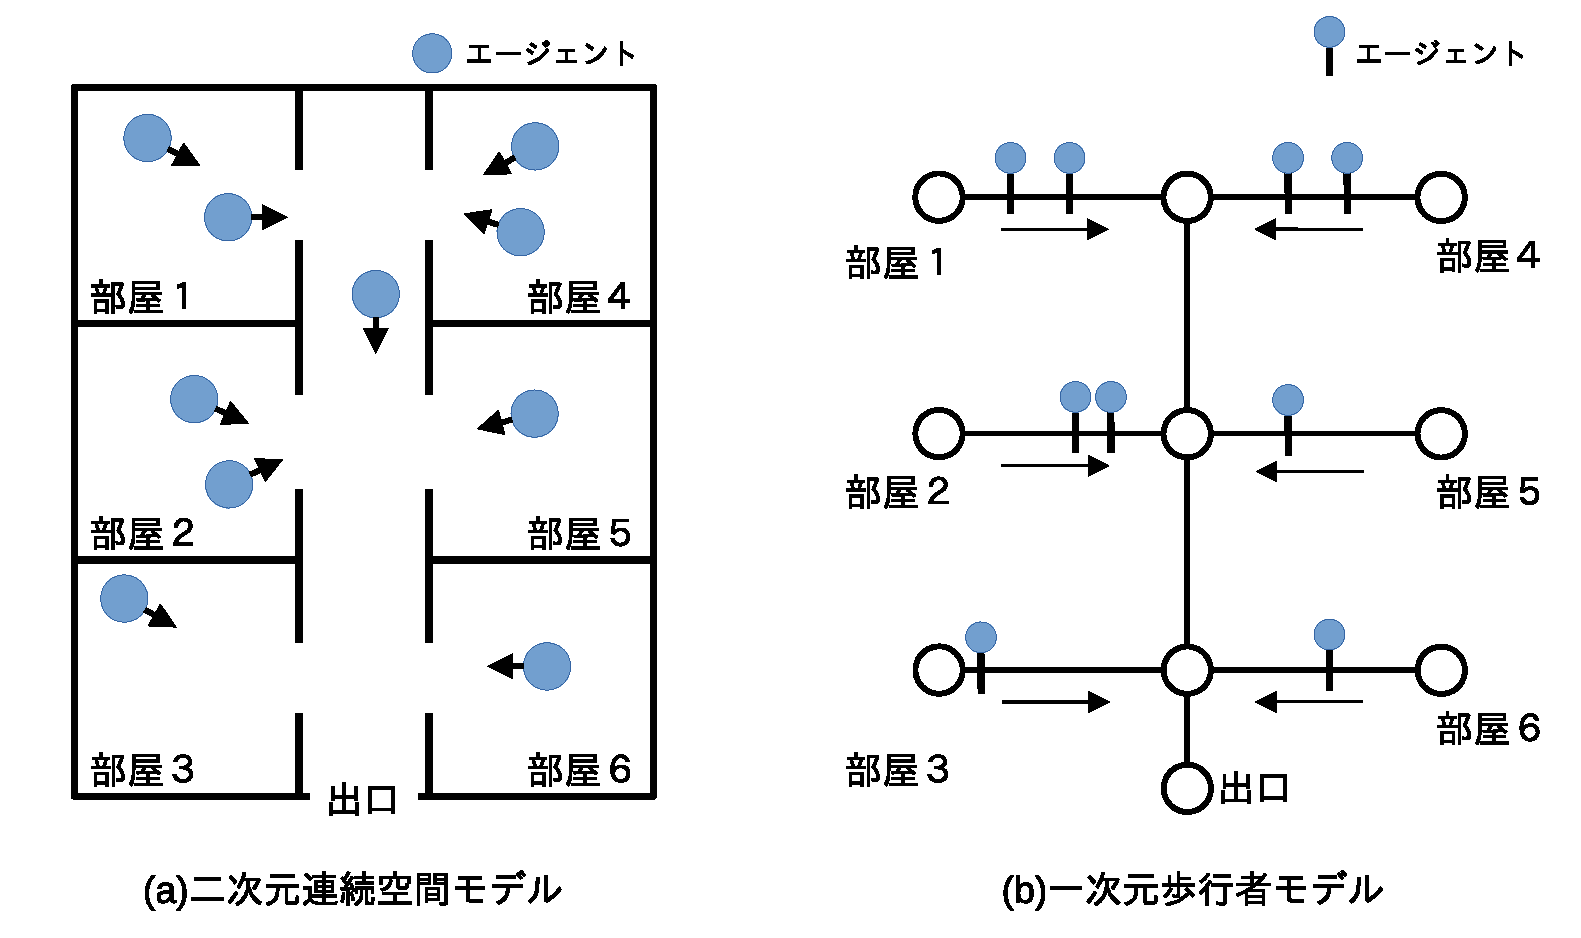
\includegraphics[width=11cm,clip]{figure/ichijigen_ex.eps}
  \caption{一次元モデルの例}
  \label{fig:ichijigen_ex}
 \end{center}
\end{figure}

\begin{figure}[hbtp]
 \begin{center}
  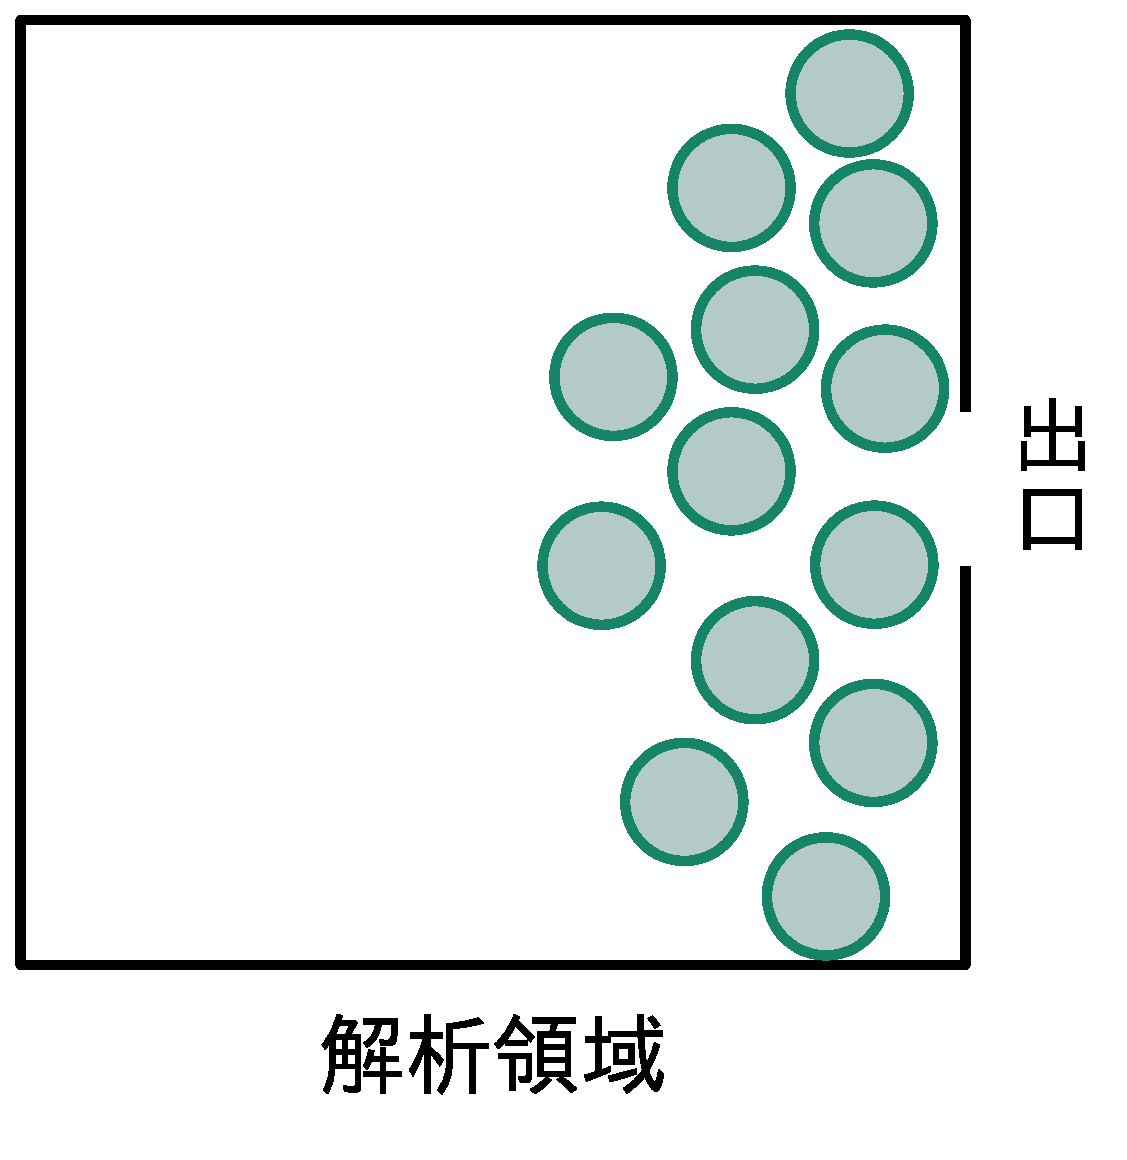
\includegraphics[width=4.5cm,clip]{figure/atigenshou.eps}
  \caption{アーチ現象の例}
  \label{fig:atigenshou}
 \end{center}
\end{figure}

\section{エージェント間の距離の計算回数削減}
SFMは,解析人数が増加するほど周囲のエージェントから受ける力の計算に
必要な周囲のエージェントが影響範囲内外かの判定の回数が増加する.
周囲のエージェントが影響範囲内外かの判定は,ルートなどを用いて
エージェント間距離$d_{ij}$を求める必要があるため,
特にエージェント間距離$d_{ij}$の計算に時間がかかる.
このため,SFMを用いた人流シミュレーションの解析時間を削減するためには,
エージェント間距離$d_{ij}$の計算回数を削減することが有効である.
エージェント間距離の計算回数削減手法にセル分割法や視野パラメータを用いた
削減手法がある.

\subsection{セル分割法}
セル分割法は,水や空気などの動きを解析できるMPS法\cite{mps}や銀河系などの圧縮性
流体に用いられるSPH法\cite{sph}などの粒子法によく用いられている.
粒子法は,近傍の粒子と相互作用する
力を計算し,粒子の行動を決定する.このため,セル分割法は,粒子法と同じように近傍の
エージェントとの相互作用力を計算するSFMに対しても用いられる.
本手法は,解析領域を格子上のセルに分割し,計算するエージェントの存在する
セルと近傍のセルに存在するエージェントに対して他のエージェントから受ける力の範囲であるか
判定し,範囲内であれば他のエージェントから受ける力を計算する手法である.
図\ref{fig:seru_ex1}にセル分割法を用いるSFMの例を示
す.図\ref{fig:seru_ex1}中の赤丸は他のエージェントから受ける力の計算をするエージ
ェント,黒丸は他のエージェント,四角は解析領域を格子状に分割したセルである.
この例では,エージェント4の行動を更新する際に青色のセル内に存在するエージェント
のみを参照するため,エージェント番号3,5,9の計算を削減できる.このとき,
視野を用いるSFMは,速度計算するエージェントの進行方向前方に存在するエージェント情報を
用いて計算するため,エージェントの進行方向後方のセルに存在するエージェント情報は不要になる,
このため,視野を用いるSFMでは,視野を考慮し,参照するセルを視野範囲に近づけることで,
計算回数を減らすことができる.

\begin{figure}[hbtp]
 \begin{center}
  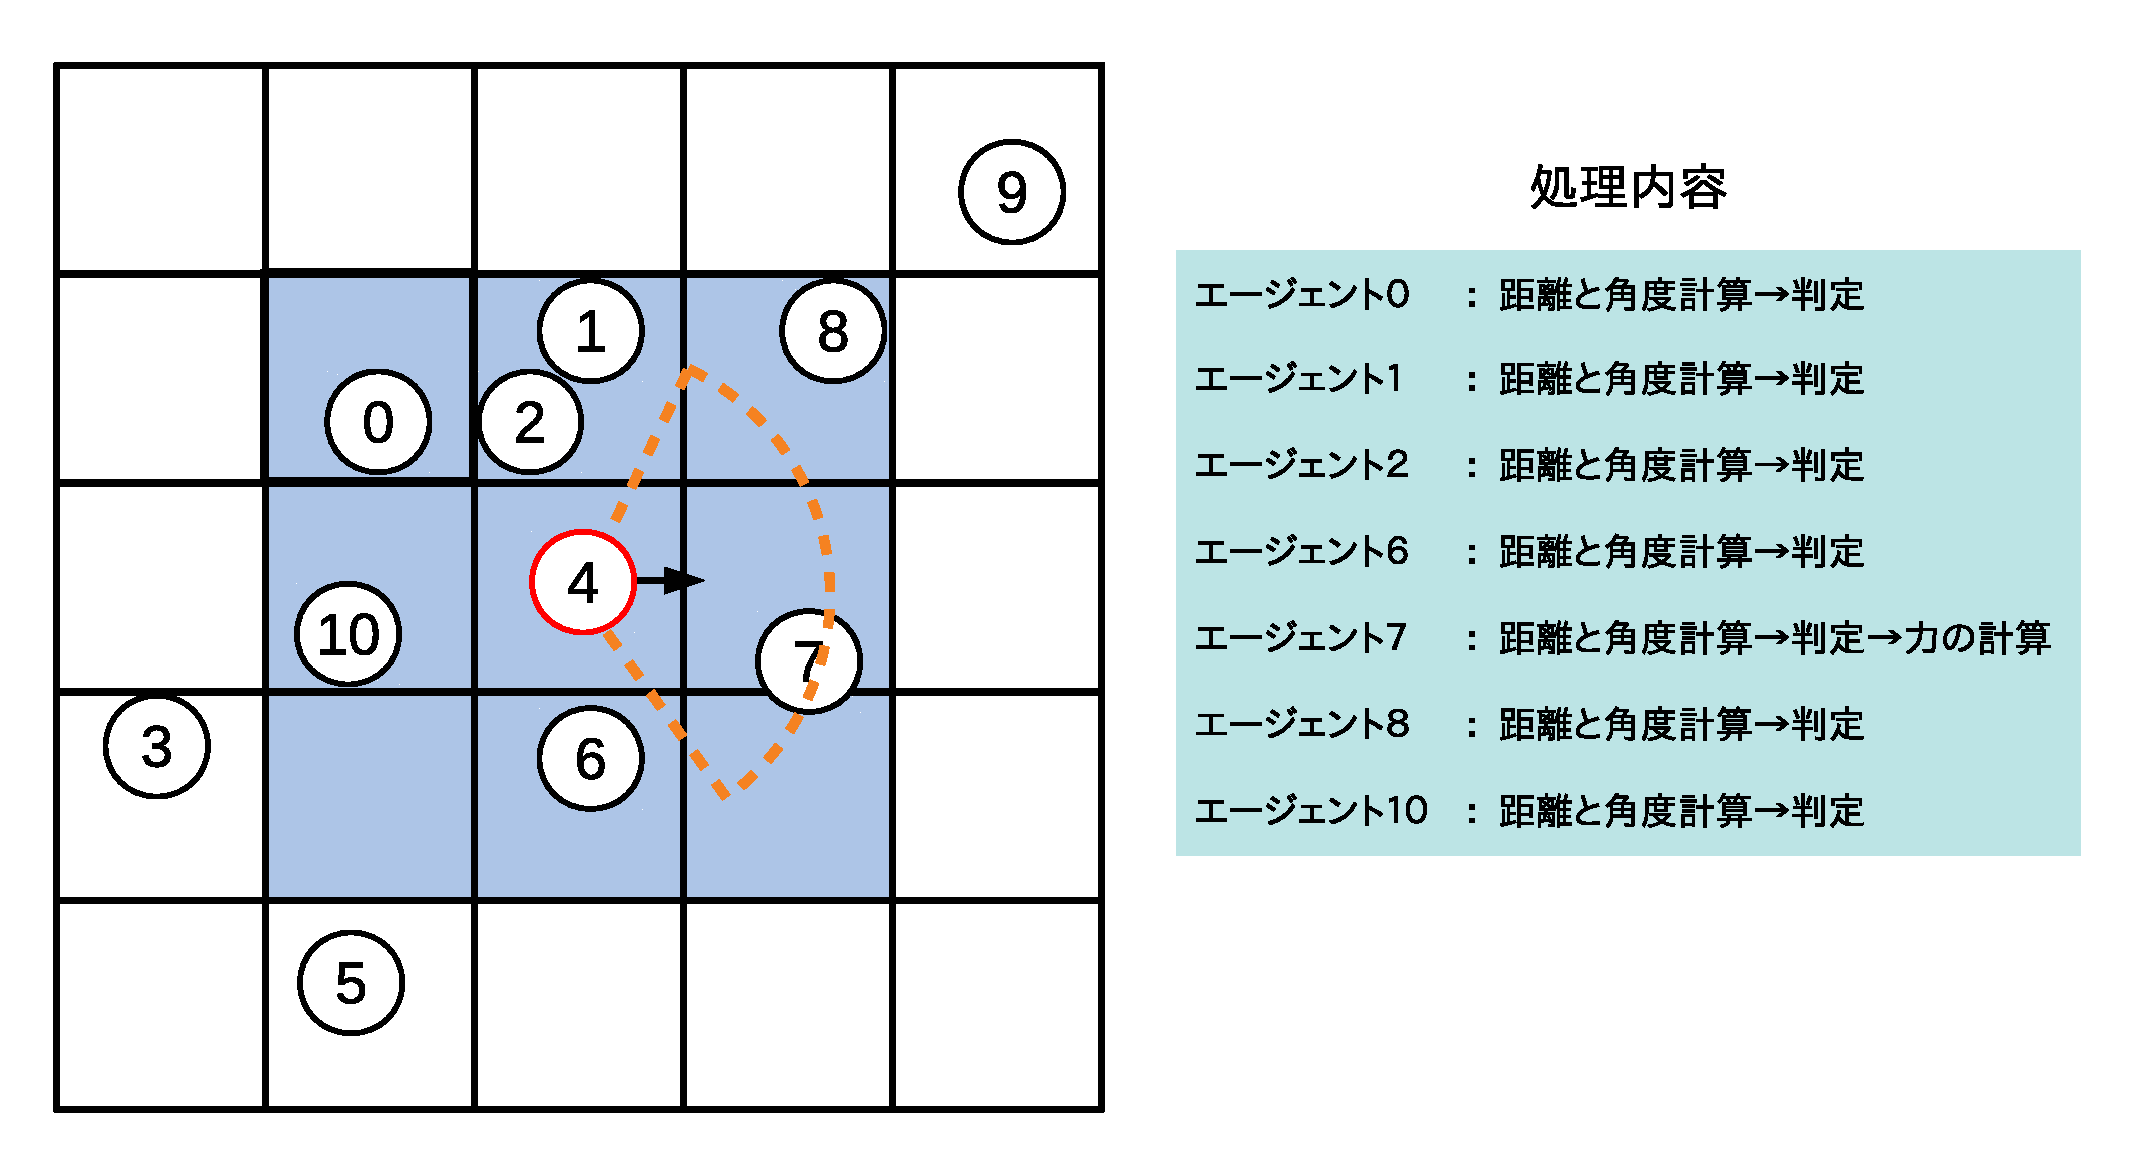
\includegraphics[width=11.5cm,clip]{figure/seru_ex1_r2.eps}
  \caption{セル分割法を用いた例}
  \label{fig:seru_ex1}
 \end{center}
\end{figure}


\subsection{視野パラメータを用いた削減手法}
視野パラメータを用いたSFMでは,


\section{単位時間あたりの計算回数}

\subsection{エージェントごとの並列性を用いた手法}

\begin{figure}[hp]
 \begin{center}
  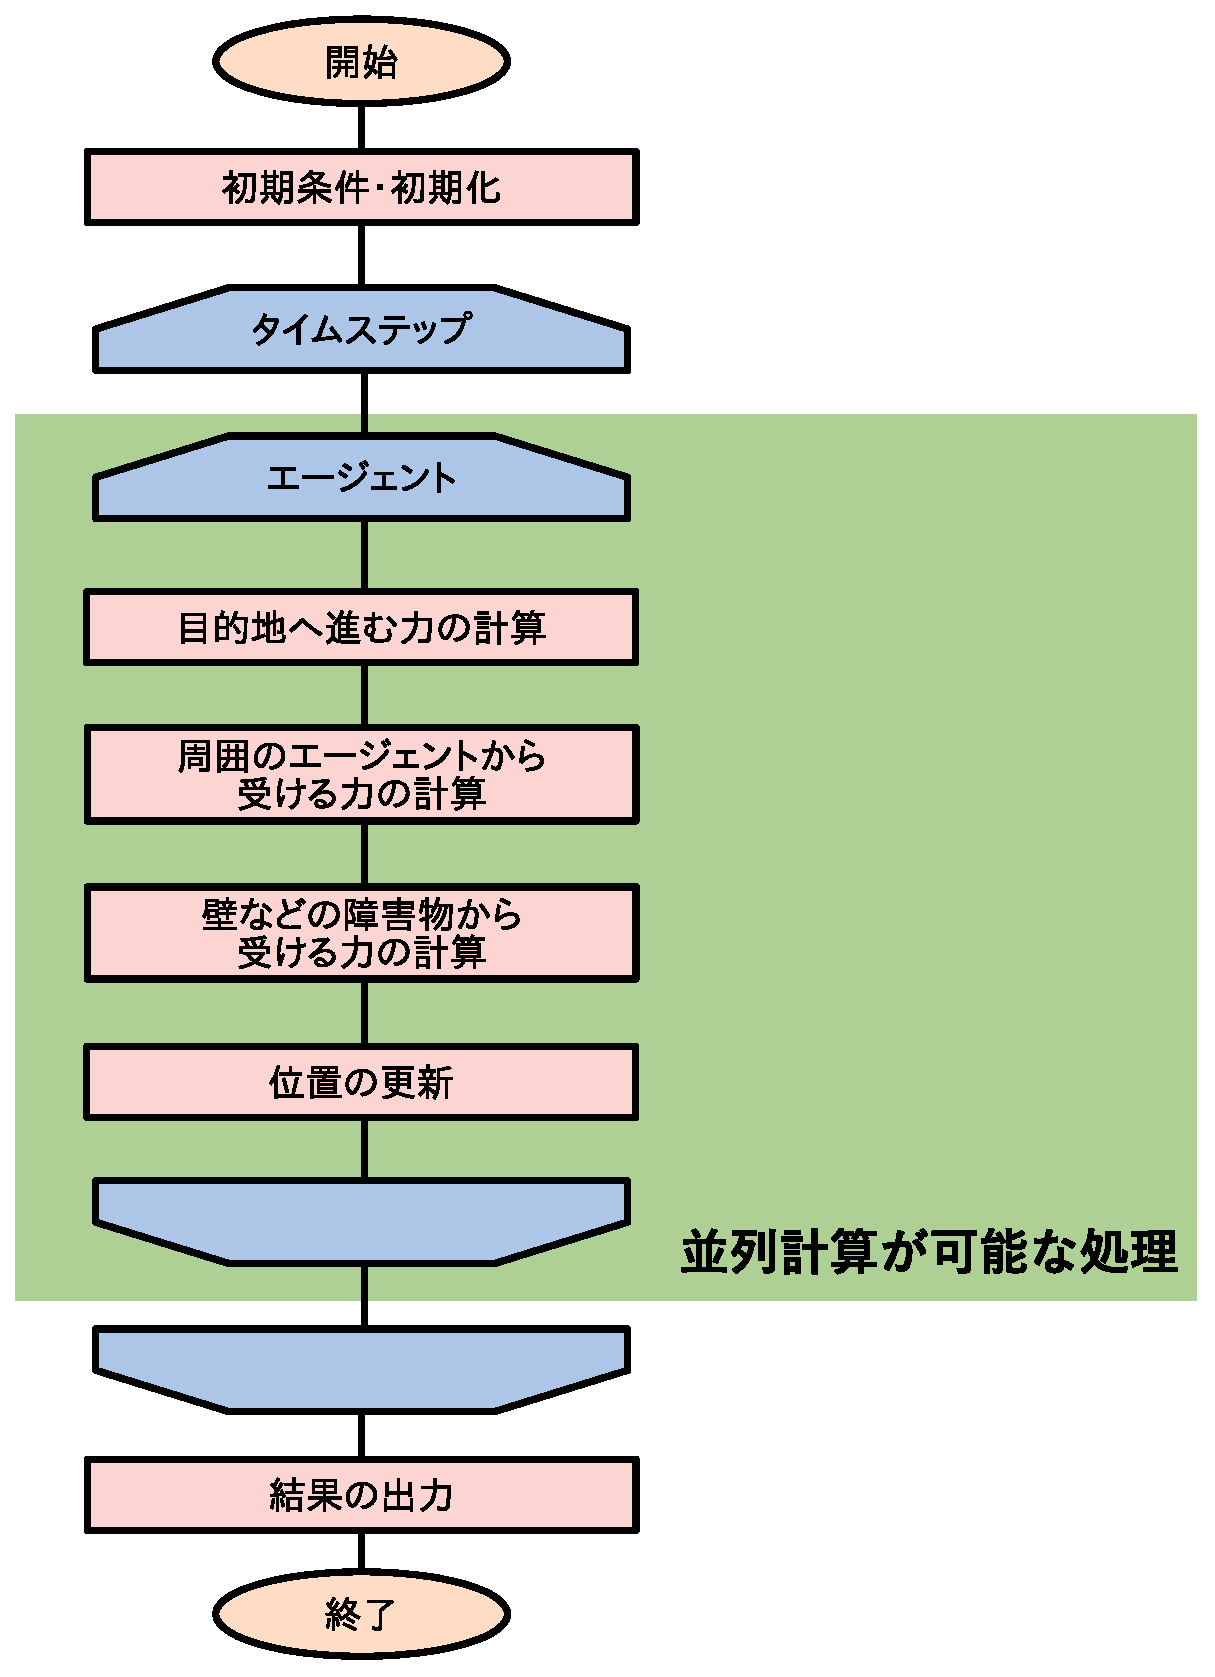
\includegraphics[width=10cm,clip]{figure/heiretuka_sfm.eps}
  \caption{SFMの並列化可能な処理}
  \label{fig:atigenshou}
 \end{center}
\end{figure}

\begin{figure}[hp]
 \begin{center}
  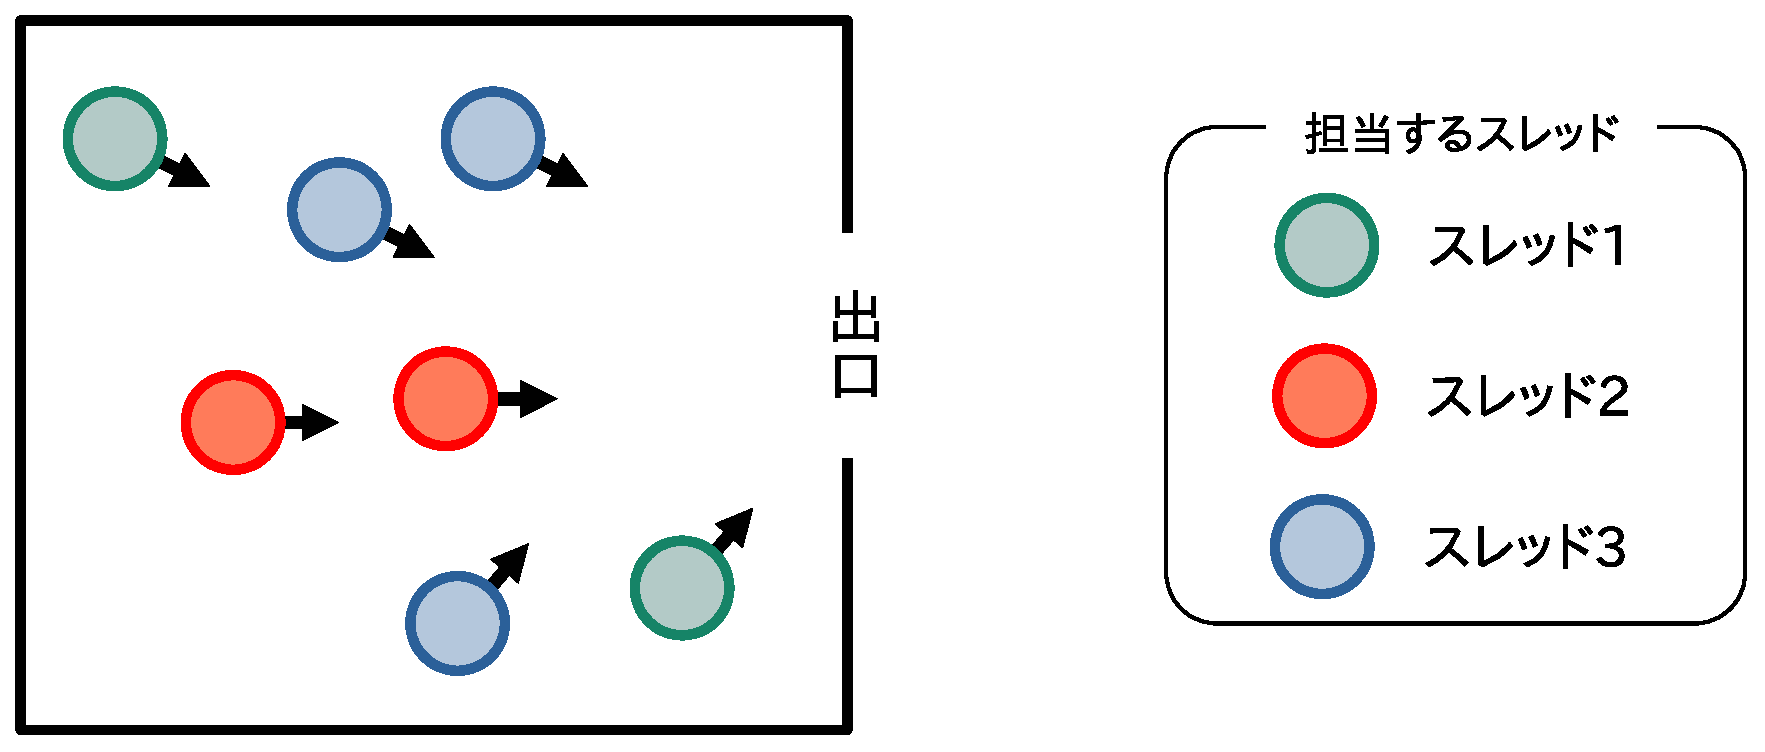
\includegraphics[width=10cm,clip]{figure/sureddo_heiretu.eps}
  \caption{3スレッドでの並列化の例}
  \label{fig:atigenshou}
 \end{center}
\end{figure}


\begin{figure}[hbtp]
 \begin{center}
  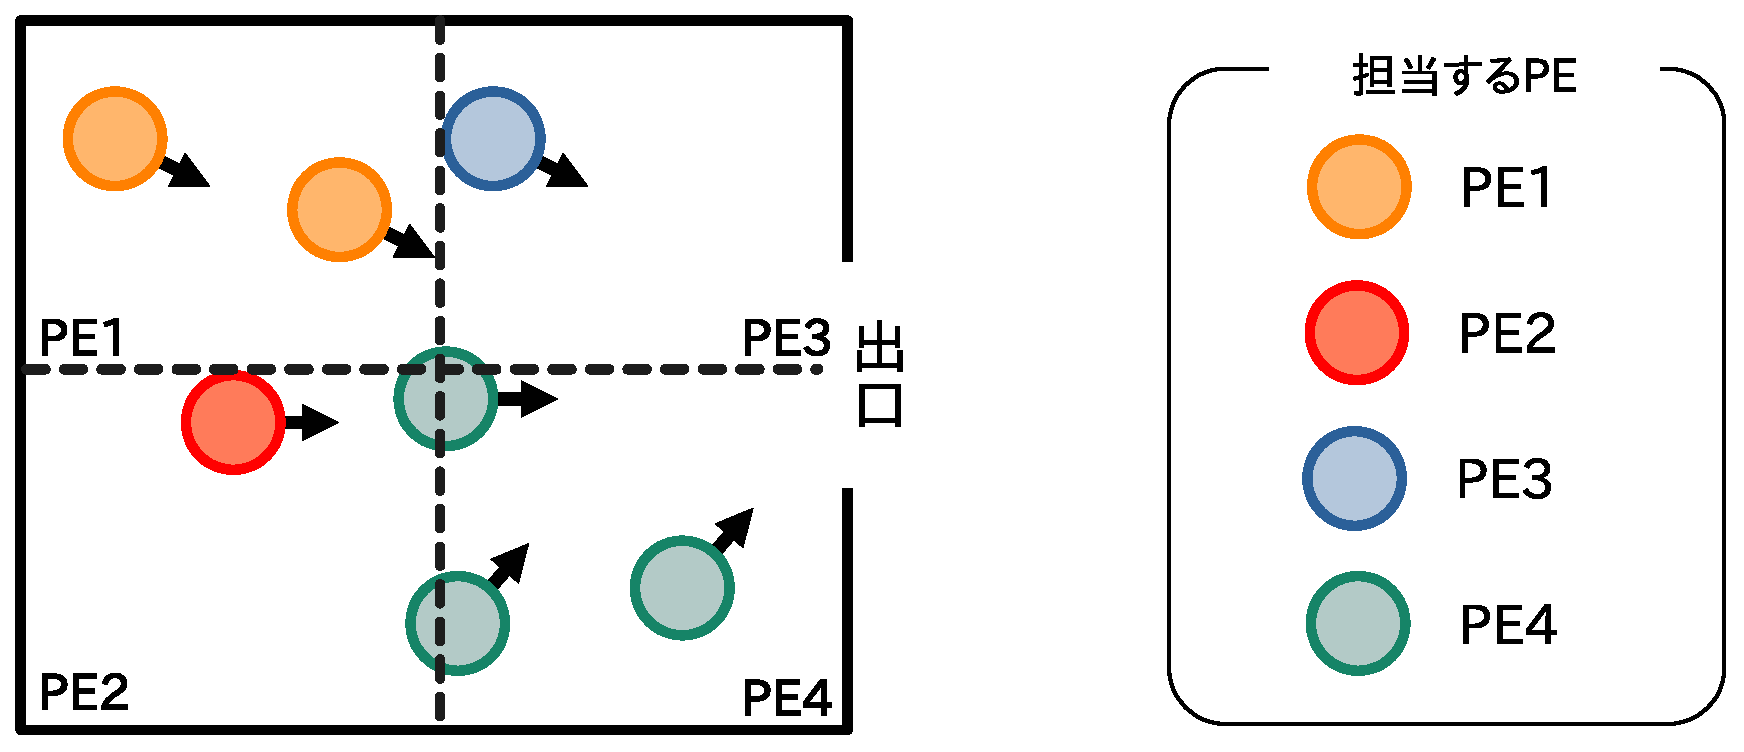
\includegraphics[width=10cm,clip]{figure/ryoiki_heiretu.eps}
  \caption{領域分割の例}
  \label{fig:atigenshou}
 \end{center}
\end{figure}


\clearpage

\subsection{解析領域ごとの並列性を用いた手法}
aaAa

\section{経路選択時の判定回数削減}
aa

\subsection{経路選択の単純化}
aa

\subsection{経路選択手法の~~}
aa

%***** END ************************************************
